\documentclass[a4paper, 12pt]{article}
% math symbols
\usepackage{amssymb}
\usepackage{amsmath}
\usepackage{mathrsfs}
\usepackage{physsummer}


\usepackage{enumitem}
\usepackage[margin = 2cm]{geometry}

\tolerance = 1000
\emergencystretch = 0.74cm



\pagestyle{empty}
\parindent = 0mm

\begin{document}

\newgeometry{margin=1.5cm}

\begin{center}
  \Large{\textbf{Городской центр физического образования, 10 класс.}\\
  \textit{Сборы к региону (эксперимент), январские каникулы.}}
\end{center}

\large

\begin{center}
  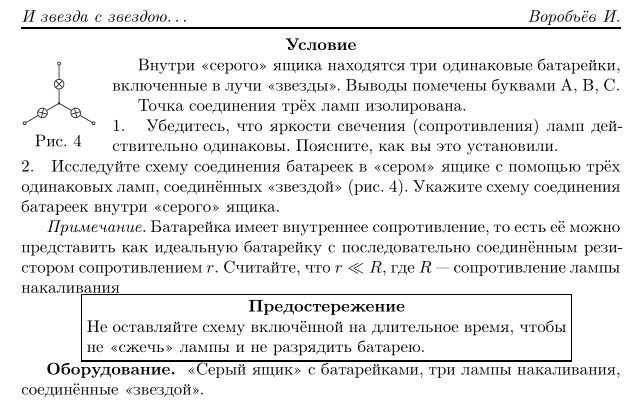
\includegraphics[width=16cm]{exp1}
  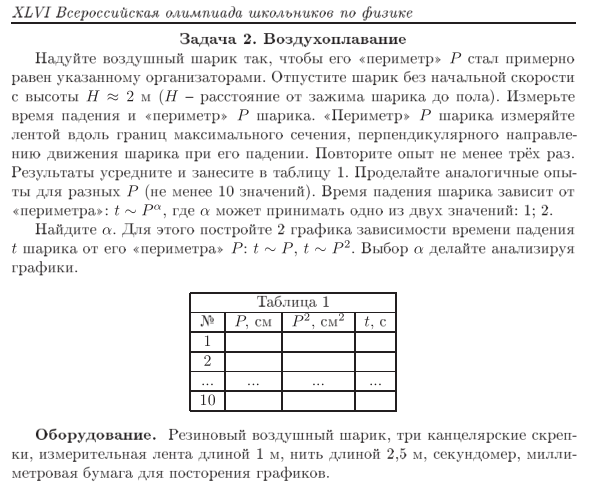
\includegraphics[width=16cm]{exp2}
\end{center}

\clearpage

\begin{center}
  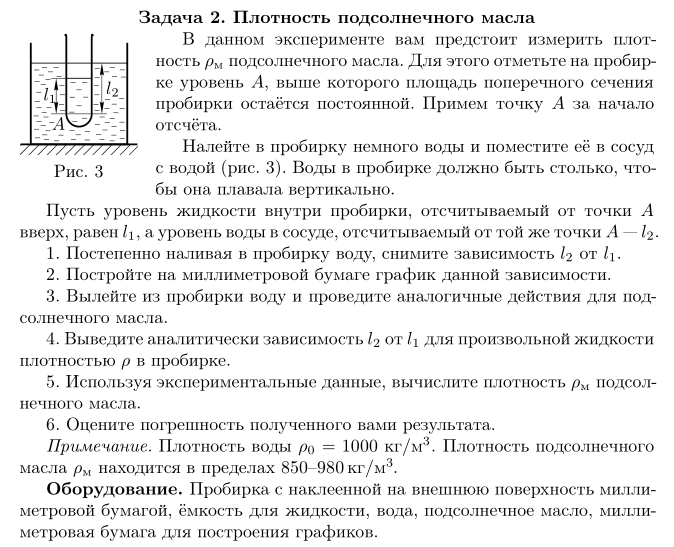
\includegraphics[width=16cm]{exp3}
  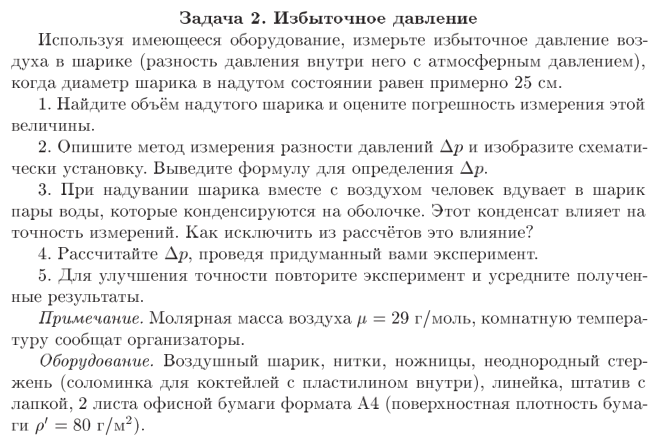
\includegraphics[width=16cm]{exp4}
\end{center}

\clearpage

\begin{center}
  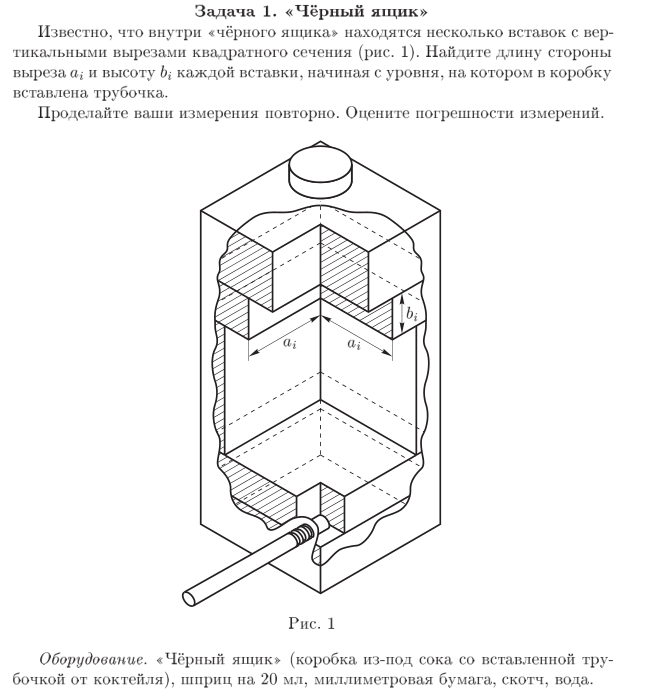
\includegraphics[width=16cm]{exp5}
  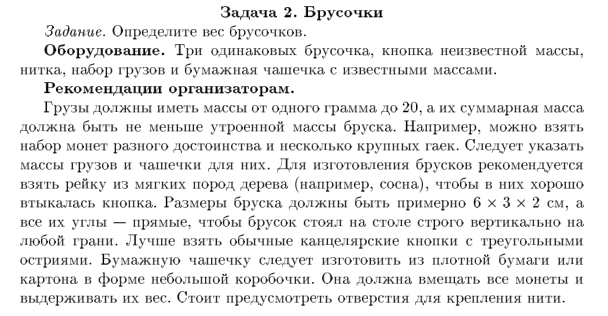
\includegraphics[width=16cm]{exp6}
\end{center}


\end{document}


%%% Local Variables: 
%%% mode: latex
%%% TeX-engine:xetex
%%% TeX-PDF-mode: t
%%% End:
